 % SampleProject.tex -- main LaTeX file for sample LaTeX article
%
%\documentclass[12pt]{article}
\documentclass[11pt]{SelfArxOneColBMN}
% add the pgf and tikz support.  This automatically loads
% xcolor so no need to load color
\usepackage{pgf}
\usepackage{tikz}
\usetikzlibrary{matrix}
\usetikzlibrary{calc}
\usepackage{xstring}
\usepackage{pbox}
\usepackage{etoolbox}
\usepackage{marginfix}
\usepackage{xparse}
\setlength{\parskip}{0pt}% fix as marginfix inserts a 1pt ghost parskip
% standard graphics support
\usepackage{graphicx,xcolor}
\usepackage{wrapfig}
%
\definecolor{color1}{RGB}{0,0,90} % Color of the article title and sections
\definecolor{color2}{RGB}{0,20,20} % Color of the boxes behind the abstract and headings
%----------------------------------------------------------------------------------------
% HYPERLINKS
%----------------------------------------------------------------------------------------
\usepackage[pdftex]{hyperref} % Required for hyperlinks
\hypersetup{hidelinks,
colorlinks,
breaklinks=true,%
urlcolor=color2,%
citecolor=color1,%
linkcolor=color1,%
bookmarksopen=false%
,pdftitle={Midterm 2},%
pdfauthor={Peterson}}
%\usepackage[round,numbers]{natbib}
\usepackage[numbers]{natbib}
\usepackage{lmodern}
\usepackage{setspace}
\usepackage{xspace}
\usepackage{pdfpages}
%
\usepackage{subfigure}
\newcommand{\goodgap}{
  \hspace{\subfigtopskip}
  \hspace{\subfigbottomskip}}
%
\usepackage{atbegshi}
%
\usepackage[hyper]{listings}
%
\usepackage{enumitem}
% use ams math packages
\usepackage{amsmath,amsthm,amssymb,amsfonts}
\usepackage{mathrsfs}
%
% use new improved Verbatim
\usepackage{fancyvrb}
%
\usepackage[titletoc,title]{appendix}
%
\usepackage{url}
%
% Create length for the baselineskip o text in footnotesize
\newdimen\footnotesizebaselineskip
\newcommand{\test}[1]{%
 \setbox0=\vbox{\footnotesize\strut Test \strut}
 \global\footnotesizebaselineskip=\ht0 \global\advance\footnotesizebaselineskip by \dp0
}
%
\usepackage{listings}

\DeclareGraphicsExtensions{.pdf, .jpg, .tif,.png}

% make sure we don't get orphaned words if at top of page
% or orphans if at bottom of page
\clubpenalty=9999
\widowpenalty=9999
\renewcommand{\textfraction}{0.15}
\renewcommand{\topfraction}{0.85}
\renewcommand{\bottomfraction}{0.85}
\renewcommand{\floatpagefraction}{0.66}
%
\DeclareMathOperator{\sech}{sech}

\newcommand{\mycite}[1]{%
(\citeauthor{#1} \citep{#1} \citeyear{#1})\xspace
}

\newcommand{\mycitetwo}[2]{%
(\citeauthor{#2} \citep[#1]{#2} \citeyear{#2})\xspace
}

\newcommand{\mycitethree}[3]{%
(\citeauthor{#3} \citep[#1][#2]{#3} \citeyear{#3})\xspace
}

\newcommand{\myincludegraphics}[3]{% file name, width, height
\includegraphics[width=#2,height=#3]{#1}
}

\newcommand{\myincludegraphicstwo}[2]{% file name, width, height
\includegraphics[scale=#1]{#2}
}

\newcommand{\mysimplegraphics}[1]{% file name, width, height
\includegraphics{#1}
}

\newcommand{\MB}[1]{
\boldsymbol{#1}
}

\newcommand{\myquotetwo}[1]{%
\small
%\singlespacing
\begin{quotation}
#1
\end{quotation}
\normalsize
%\onehalfspacing  
}

\newcommand{\jimquote}[1]{%
\small
%\singlespacing
\begin{quotation}
#1
\end{quotation}
\normalsize
%\onehalfspacing
}

\newcommand{\myquote}[1]{%
\small
%\singlespacing
\begin{quotation}
#1
\end{quotation}
\normalsize
%\onehalfspacing  
}

%A =
%
%[2 r_1 	     r_1]
%[-2r_1 + r_2  r_2 - r_1]
%
%has eigenvalues r_1 neq r_2.
% #1 = 2 r_1, #2 = r_1, #3 = -2r_1+r_2, #4 = r_2 - r_1
\newcommand{\myrealdiffA}[4]{
\left [
\begin{array}{rr}
#1  & #2\\
#3  & #4
\end{array}
\right ]
}

% args:
% 1, 2 ,3, 4, 5 = caption, label, width, height, file name
%\mysubfigure{}{}{}{}{}
\newcommand{\mysubfigure}[5]{%
\subfigure[#1]{\label{#2}\includegraphics[width=#3,height=#4]{#5}}
}

\newcommand{\mysubfiguretwo}[3]{%
\subfigure[#1]{\label{#2}\includegraphics{#3}}
}

\newcommand{\mysubfigurethree}[4]{%
\subfigure[#1]{\label{#2}\includegraphics[scale=#3]{#4}}
}

\newcommand{\myputimage}[5]{% file name, width, height
\centering
\includegraphics[width=#3,height=#4]{#5}
\caption{#1}
\label{#2}
}

\newcommand{\myputimagetwo}[4]{% caption, label, scale, file name
\centering
\includegraphics[scale=#3]{#4}
\caption{#1}
\label{#2}
}

\newcommand{\myrotateimage}[5]{% file name, width, height
\centering
\includegraphics[scale=#3,angle=#4]{#5}
\caption{#1}
\label{#2}
}

\newcommand{\myurl}[2]{%
\href{#1}{\bf #2}
}

\RecustomVerbatimEnvironment%
{Verbatim}{Verbatim}  
  {fillcolor=\color{black!20}}
  
  \DefineVerbatimEnvironment%
{MyVerbatim}{Verbatim}  
  {frame=single,
   framerule=2pt,
   fillcolor=\color{black!20},
   fontsize=\small}
   
\newcommand{\myfvset}[1]{%  
\fvset{frame=single,
       framerule=2pt,
       fontsize=\small,
       xleftmargin=#1in}}
       
\newcommand{\mylistverbatim}{%
\lstset{%
  fancyvrb, 
  basicstyle=\small,
  breaklines=true}
}  

\newcommand{\mylstinlinebf}[1]{%
{\bf #1}
}

\newcommand{\mylstinline}{%
\lstset{%
  basicstyle=\color{black!80}\bfseries\ttfamily,
  showstringspaces=false,
  showspaces=false,showtabs=false,
  breaklines=true}
\lstinline
}

\newcommand{\mylstinlinetwo}[1]{%
\lstset{%
  basicstyle=\color{black!80}\bfseries\ttfamily,
  showstringspaces=false,
  showspaces=false,showtabs=false,
  breaklines=true}
\lstinline!#1! 
}

%fontfamily=tt
%fontfamily=courier
%fontfamily=helvetica
%frame=topline,
%frame=single,
 %frame=lines,
 %framesep=10pt,
 %fontshape=it,
 %fontseries=b,
 %fontsize=\relsize{-1},
 %fillcolor=\color{black!20},
 %rulecolor=\color{yellow},
 %fillcolor=\color{red}
 %label=\fbox{\Large\emph{The code}}
\DefineVerbatimEnvironment%
{MyListVerbatim}{Verbatim}  
{
fillcolor=\color{black!10},
fontfamily=courier,
frame=single,
%formatcom=\color{white},
framesep=5mm,
labelposition=topline,
fontshape=it,
fontseries=b,
fontsize=\small,
label=\fbox{\large\emph{The code}\normalsize}
} 

%  caption={[#1] \large\bf{#1}}, 
%\centering \framebox[.6\textwidth][c]{\Large\bf{#1}}
\newcommand{\myfancyverbatim}[1]{%
\lstset{%
  fancyvrb=true, 
  %fvcmdparams= fillcolor 1,
  %morefvcmdparams = \textcolor 2,
  frame=shadowbox,framerule=2pt, 
  basicstyle=\small\bfseries,
  backgroundcolor=\color{black!08},
  showstringspaces=false,
  showspaces=false,showtabs=false,
  keywordstyle=\color{black}\bfseries,
  %numbers=left,numberstyle=\tiny,stepnumber=5,numbersep=5pt,
  stringstyle=\ttfamily,
  caption={[\quad #1] \mbox{}\\ \vspace{0.1in} \framebox{\large \bf{#1} \small} },  
  belowcaptionskip=20 pt,  
  label={},
  xleftmargin=17pt,
  framexleftmargin=17pt,
  framexrightmargin=5pt,
  framexbottommargin=4pt,
  nolol=false,
  breaklines=true}
}

\newcommand{\mylistcode}[3]{%
\lstset{%
  language=#1, 
  frame=shadowbox,framerule=2pt, 
  basicstyle=\small\bfseries,
  backgroundcolor=\color{black!16},
  showstringspaces=false,
  showspaces=false,showtabs=false,
  keywordstyle=\color{black!40}\bfseries,
  numbers=left,numberstyle=\tiny,stepnumber=5,numbersep=5pt,
  stringstyle=\ttfamily,
  caption={[\quad#2] \mbox{}\\ \vspace{0.1in} \framebox{\large \bf{#2} \small} },
  belowcaptionskip=20 pt,
  breaklines=true,
  xleftmargin=17pt,
  framexleftmargin=17pt,
  framexrightmargin=5pt,
  framexbottommargin=4pt,  
  label=#3,
  breaklines=true} 
}

  %caption={[#2] #3},
  %caption={[#2]{\mbox{}\\ \vspace{0.1in} \framebox{\large \bf{#3} \small}},
  %caption={[#2] \mbox{}\\ \bf{#3} },

% frame=single,
% caption={[Code Fragment] {\bf Code Fragment} },
% caption={[Code Fragment] \mbox{}\\ \vspace{0.1in} \framebox{\large \bf{Code Fragment} \small} },
\newcommand{\mylistcodequick}[1]{%
\lstset{%
  language=#1, 
  frame=shadowbox,framerule=2pt, 
  basicstyle=\small\bfseries,
  backgroundcolor=\color{black!16},
  showstringspaces=false,
  showspaces=false,showtabs=false,
  keywordstyle=\color{black!40}\bfseries,
  numbers=left,numberstyle=\tiny,stepnumber=5,numbersep=5pt,
  stringstyle=\ttfamily,
  caption={[\quad Code Fragment] \large \bf{Code Fragment} \small},   
  belowcaptionskip=20 pt,  
  label={},
  xleftmargin=17pt,
  framexleftmargin=17pt,
  framexrightmargin=5pt,
  framexbottommargin=4pt,
  breaklines=true} 
}

%  caption={[#2] \mbox{}\\ \vspace{0.1in} \framebox{\large \bf{#2} \small} },
\newcommand{\mylistcodequicktwo}[2]{%
\lstset{%
  language=#1, 
  frame=shadowbox,framerule=2pt, 
  basicstyle=\small\bfseries,
  extendedchars=true,
  backgroundcolor=\color{black!16},
  showstringspaces=false,
  showspaces=false,
  showtabs=false,
  keywordstyle=\color{black!40}\bfseries,
  numbers=left,numberstyle=\tiny,stepnumber=5,numbersep=5pt,
  stringstyle=\ttfamily,
  caption={[\quad#2] \large \bf{#2} \small},
  belowcaptionskip=20 pt,
  label={},
  xleftmargin=17pt,
  framexleftmargin=17pt,
  framexrightmargin=5pt,
  framexbottommargin=4pt,
  breaklines=true} 
}

%  caption={[#2] \mbox{}\\ \vspace{0.1in} \framebox{\large \bf{#2} \small} },
\newcommand{\mylistcodequickthree}[2]{%
\lstset{%
  language=#1, 
  frame=shadowbox,framerule=2pt, 
  basicstyle=\small\bfseries,
  extendedchars=true,
  backgroundcolor=\color{black!16},
  showstringspaces=false,
  showspaces=false,
  showtabs=false,
  keywordstyle=\color{black!40}\bfseries,
  numbers=left,numberstyle=\tiny,stepnumber=5,numbersep=5pt,
  stringstyle=\ttfamily,
  caption={[\quad#2] \large\bf{#2}\small},
  belowcaptionskip=20 pt,
  label={},
  xleftmargin=17pt,
  framexleftmargin=17pt,
  framexrightmargin=5pt,
  framexbottommargin=4pt,
  breaklines=true} 
}

%  frame=single,
\newcommand{\mylistset}[4]{%
\lstset{language=#1,
  basicstyle=\small,
  showstringspaces=false,
  showspaces=false,showtabs=false,
  keywordstyle=\color{black!40}\bfseries,
  numbers=left,numberstyle=\tiny,stepnumber=5,numbersep=5pt,
  stringstyle=\ttfamily,
  caption={[\quad#2]#3},
  label=#4}
}

\newcommand{\mylstinlineset}{%
\lstset{%
  basicstyle=\color{blue}\bfseries\ttfamily,
  showstringspaces=false,
  showspaces=false,showtabs=false,
  breaklines=true}
}

\newcommand{\myframedtext}[1]{%
\centering
\noindent
%\fbox{\parbox[c]{.9\textwidth}{\color{black!40} \small \singlespacing #1\onehalfspacing \normalsize \\}}
\fbox{\parbox[c]{.9\textwidth}{\color{black!40} \small  #1 \normalsize \\}}
}

\newcommand{\myemptybox}[2]{% from , to
\fbox{\begin{minipage}[t][#1in][c]{#2in}\hspace{#2in}\end{minipage}}
}

\newcommand{\myemptyboxtwo}[2]{% from , to
\centering\fbox{
\begin{minipage}{#1in}
\hfill\vspace{#2in}
\end{minipage}
}
}

\newcommand{\boldvector}[1]{
\boldsymbol{#1}
}

\newcommand{\dEdY}[2]{\frac{d E}{d Y_{#1}^{#2}}}
\newcommand{\dEdy}[2]{\frac{d E}{d y_{#1}^{#2}}}
\newcommand{\dEdT}[2]{\frac{\partial E}{\partial T_{{#1} \rightarrow {#2}}}}
\newcommand{\dEdo}[1]{\frac{\partial E}{\partial o^{#1}}}
\newcommand{\dEdg}[1]{\frac{\partial E}{\partial g^{#1}}}
\newcommand{\dYdY}[4]{\frac{\partial Y_{#1}^{#2}}{\partial Y_{#3}^{#4}}}
\newcommand{\dYdy}[4]{\frac{\partial Y_{#1}^{#2}}{\partial y_{#3}^{#4}}}
\newcommand{\dydY}[4]{\frac{\partial y_{#1}^{#2}}{\partial Y_{#3}^{#4}}}
\newcommand{\dydy}[4]{\frac{\partial y_{#1}^{#2}}{\partial y_{#3}^{#4}}}
\newcommand{\dydT}[4]{\frac{\partial y_{#1}^{#2}}{\partial T_{{#3} \rightarrow {#4}}}}
\newcommand{\dYdT}[4]{\frac{\partial Y_{#1}^{#2}}{\partial T_{{#3} \rightarrow {#4}}}}
\newcommand{\dTdT}[4]{\frac{\partial T_{{#1} \rightarrow {#2}}}{\partial T_{{#3} \rightarrow {#4}}}}
\newcommand{\ssum}[2]{\sum_{#1}^{#2}}

\newcommand{\ssty}[1]{\scriptscriptstyle #1}

\newcommand{\myparbox}[2]{%
\parbox{#1}{\color{black!20} #2}
}

\newcommand{\bs}[1]{
\boldsymbol{#1}
}

\newcommand{\parone}[2]{%
\frac{\partial #1 }{ \partial #2 }
}
\newcommand{\partwo}[2]{%
\frac{ \partial^2 {#1} }{ \partial {#2}^2 }
}

\newcommand{\twodvectorvarfun}[2]{
\left [
\begin{array}{r}
{{#1_{\ssty{1}}}(#2)} \\
{{#1_{\ssty{2}}}(#2)}
\end{array}
\right ]
}
\newcommand{\twodvectorvarprimed}[1]{
\left [
\begin{array}{r}
{{#1_{\ssty{1}}}'(t)} \\
{{#1_{\ssty{2}}}'(t)}
\end{array}
\right ]
}

\newcommand{\complex}[2]{#1 \: #2 \: \boldsymbol{i}}
\newcommand{\complexmag}[2]%
{
\sqrt{(#1)^2 \: + \: (#2)^2}
}
\newcommand{\threenorm}[3]%
{
\sqrt{(#1)^2 \: + \: (#2)^2 \: + \: (#3)^2}
}
\newcommand{\norm}[1]{\mid \mid #1 \mid \mid}

\newcommand{\myderiv}[2]{\frac{d #1}{d #2}}
\newcommand{\myderivb}[2]{\frac{d}{d #2} \left ( #1 \right )}
\newcommand{\myrate}[3]%
{#1^\prime(#2) &=& #3 \: #1(#2)
}
\newcommand{\myrateexter}[4]%
{#1^\prime(#2) &=& #3 \: #1(#2) \: + \: #4
}
\newcommand{\myrateic}[3]%
{#1( \: #2 \:) &=& #3 
}

\newcommand{\mytwodsystemeqn}[6]{
#1 \: x    #2 \: y &=& #3\\
#4 \: x    #5 \: y &=& #6\\
}

\newcommand{\mytwodsystem}[8]{
#3 \: #1 \: + \: #4 \: #2 &=& #5\\
#6 \: #1 \: + \: #7 \: #2 &=& #8\\
}  

\newcommand{\mytwodarray}[4]{
\left [
\begin{array}{rr}
#1 & #2\\
#3 & #4
\end{array}
\right ]
}

\newcommand{\mytwoid}{
\left [
\begin{array}{rr}
1 & 0\\
0 & 1
\end{array}
\right ]
}

\newcommand{\myxprime}[2]{
\left [
\begin{array}{r}
#1^\prime(t)\\
#2^\prime(t)
\end{array}
\right ]
}

\newcommand{\myxprimepacked}[2]{
\left [
\begin{array}{r}
#1^\prime\\
#2^\prime
\end{array}
\right ]
}

\newcommand{\myx}[2]{
\left [
\begin{array}{r}
#1(t)\\
#2(t)
\end{array}
\right ]
}

\newcommand{\myxonly}[2]{
\left [
\begin{array}{r}
#1\\
#2
\end{array}
\right ]
}

\newcommand{\myv}[2]{
\left [
\begin{array}{r}
#1\\
#2
\end{array}
\right ]
}

\newcommand{\myxinitial}[2]{
\left [
\begin{array}{r}
#1(0)\\
#2(0)
\end{array}
\right ]
}

\newcommand{\twodboldv}[1]{
\boldsymbol{#1}
}

\newcommand{\mytwodvector}[2]{
\left [
\begin{array}{r}
#1\\
#2
\end{array}
\right ]
}

\newcommand{\mythreedvector}[3]{
\left [
\begin{array}{r}
#1\\
#2\\
#3
\end{array}
\right ]
}

\newcommand{\mytwodsystemvector}[6]{
\left [
\begin{array}{rr}
#1 & #2\\
#4 & #5
\end{array}
\right ]
\:
\left [
\begin{array}{r}
x \\
y 
\end{array}
\right ]
&=&
\left [
\begin{array}{r}
#3\\
#6
\end{array}
\right ]
}

\newcommand{\mythreedarray}[9]{
\left [
\begin{array}{rrr}
#1 & #2 & #3\\
#4 & #5 & #6\\
#7 & #8 & #9
\end{array}
\right ]
}

\newcommand{\myodetwo}[6]{
#1 \: #6^{\prime \prime}(t) \: #2 \: #6^{\prime}(t) \: #3 \: #6(t) &=& 0\\
#6(0)                                           &=& #4\\
#6^{\prime}(0)                                  &=& #5
}

\newcommand{\myodetwoNoIC}[4]{
#1 \: #4^{\prime \prime}(t) \: #2 \: #4^{\prime}(t) \: #3 \: #4(t) &=& 0
}

\newcommand{\myodetwopacked}[5]{
\hspace{-0.3in}& & #1 u^{\prime \prime} #2 u^{\prime} #3 u \: = \: 0\\
\hspace{-0.3in}& & u(0) \: = \: #4, \: \: u^{\prime}(0)    \: = \:  #5
}

\newcommand{\myodetwoforced}[6]{
#1\: u^{\prime \prime}(t) \: #2 \: u^{\prime}(t) \: #3 \: u(t) &=& #6\\
u(0)                                           &=& #4\\
u^{\prime}(0)                                  &=& #5\\
}

\newcommand{\myodesystemtwo}[8]{
#1 \: x^\prime(t) \: #2 \: y^\prime(t) \: #3 \: x(t) \: #4 \: y(t) &=& 0\\
#5 \: x^\prime(t) \: #6 \: y^\prime(t) \: #7 \: x(t) \: #8 \: y(t) &=& 0\\
}

\newcommand{\myodesystemtwoic}[2]{
x(0)                                       &=& #1\\ 
y(0)                                       &=& #2
}

\newcommand{\mypredprey}[4]{
x^\prime(t) &=& #1 \: x(t) \: - \: #2 \: x(t) \: y(t)\\
y^\prime(t) &=& -#3 \: y(t) \: + \: #4 \: x(t) \: y(t)
}

\newcommand{\mypredpreypacked}[4]{
x^\prime &=& #1 \: x - #2 \: x \: y\\
y^\prime &=& -#3 \: y + #4 \: x \: y
}

\newcommand{\mypredpreyself}[6]{
x^\prime(t) &=&  #1 \: x(t) \: - \: #2 \: x(t) \: y(t) \: - \: #3 \: x(t)^2\\
y^\prime(t) &=& -#4 \: y(t) \: + \: #5 \: x(t) \: y(t) \: - \: #6 \: y(t)^2
}

\newcommand{\mypredpreyfish}[5]{
x^\prime(t) &=&  #1 \: x(t) \: - \: #2 \: x(t) \: y(t) \: - \: #5 \: x(t)\\
y^\prime(t) &=& -#3 \: y(t) \: + \: #4 \: x(t) \: y(t) \: - \: #5 \: y(t)
}

\newcommand{\myepidemic}[4]{
S^\prime(t) &=& - #1 \: S(t) \: I(t)\\
I^\prime(t) &=&   #1 \: S(t) \: I(t) \: - \: #2 \: I(t)\\
S(0)        &=&   #3\\
I(0)        &=&   #4\\
}

\newcommand{\bsred}[1]{%
\textcolor{red}{\boldsymbol{#1}}
}

\newcommand{\bsblue}[1]{%
\textcolor{blue}{\boldsymbol{#1}}
}


\newcommand{\myfloor}[1]{%
\lfloor{#1}\rfloor
}

\newcommand{\cubeface}[7]{%
\begin{bmatrix}
\bs{#3}          & \longrightarrow & \bs{#4}\\
\uparrow          &                         &  \uparrow  \\
\bs{#1} & \longrightarrow & \bs{#2}\\
              & \text{ \bfseries #5:} \: \bs{#6} \: \text{\bfseries  #7 } & 
\end{bmatrix}
}

\newcommand{\cubefacetwo}[5]{%
\begin{bmatrix}
\bs{#3}          & \longrightarrow & \bs{#4}\\
\uparrow          &                         &  \uparrow  \\
\bs{#1} & \longrightarrow & \bs{#2}\\
              & \text{ \bfseries #5} & 
\end{bmatrix}
}

\newcommand{\cubefacethree}[9]{%
\begin{bmatrix}
\bs{#3}                  & \overset{#9}{\longrightarrow} & \bs{#4}\\
\uparrow \: #7         &                                             &  \uparrow  \: #8 \\
\bs{#1}                  & \overset{#6}{\longrightarrow} & \bs{#2}\\
                               & \text{ \bfseries #5} & 
\end{bmatrix}
}

\renewcommand{\qedsymbol}{\hfill \blacksquare}
\newcommand{\subqedsymbol}{\hfill \Box}
%\theoremstyle{plain}

\newtheoremstyle{mystyle}% name
  {6pt}%      Space above
  {6pt}%      Space below
  {\itshape}%         Body font
  {}%         Indent amount (empty = no indent, \parindent = para indent)
  {\bfseries}% Thm head font
  {}%        Punctuation after thm head
  { }%     Space after thm head: " " = normal interword space; \newline = linebreak
  {}%         Thm head spec (can be left empty, meaning `normal')
\theoremstyle{mystyle}
 
\newtheorem{axiom}{Axiom}
%\newtheorem{solution}{Solution}[section]
\newtheorem*{solution}{Solution}
\newtheorem{exercise}{Exercise}[section]
\newtheorem{theorem}{Theorem}[section]
\newtheorem{proposition}[theorem]{Proposition}
\newtheorem{prop}[theorem]{Proposition}
\newtheorem{assumption}{Assumption}[section]
\newtheorem{definition}{Definition}[section]
\newtheorem{comment}{Comment}[section]
\newtheorem*{question}{Question}
\newtheorem{program}{Program}[section]
%\newtheorem{myproof}{Proof}
%\newtheorem*{myproof}{Proof}[section]
\newtheorem{myproof}{Proof}[section]
\newtheorem{hint}{Hint}[section]
\newtheorem*{phint}{Hint}
\newtheorem{lemma}[theorem]{Lemma}
\newtheorem{example}{Example}[section]
      
\newenvironment{myassumption}[4]
{
\centering
\begin{assumption}[{\textbf{#1}\nopunct}]%
\index{#2}
\mbox{}\\  \vskip6pt \colorbox{black!15}{\fbox{\parbox{.9\textwidth}{#3}}}
\label{#4}
\end{assumption}
%\renewcommand{\theproposition}{\arabic{chapter}.\arabic{section}.\arabic{assumption}} 
}%
{}

\newenvironment{myproposition}[4]
{
\centering
\begin{proposition}[{\textbf{#1}\nopunct}]%
\index{#2} 
\mbox{}\\  \vskip6pt \colorbox{black!15}{\fbox{\parbox{.9\textwidth}{#3}}}
\label{#4}
\end{proposition}
%\renewcommand{\theproposition}{\arabic{chapter}.\arabic{section}.\arabic{proposition}} 
}%
{}

\newenvironment{mytheorem}[4]
{
\centering
\begin{theorem}[{\textbf{#1}\nopunct}]%
\index{#2} 
\mbox{}\\ \vskip6pt \colorbox{black!15}{\fbox{\parbox{.9\textwidth}{#3}}}
\label{#4}
\end{theorem}
%\renewcommand{\thetheorem}{\arabic{chapter}.\arabic{section}.\arabic{theorem}} 
}%
{}

\newenvironment{mydefinition}[4]
{
\centering
\begin{definition}[{\textbf{#1}\nopunct}]%
\index{#2} 
\mbox{}\\  \vskip6pt \colorbox{black!15}{\fbox{\parbox{.9\textwidth}{#3}}}
\label{#4}
\end{definition}
%\renewcommand{\thedefinitio{n}{\arabic{chapter}.\arabic{section}.\arabic{definition}} 
}%
{}

\newenvironment{myaxiom}[4]
{
\centering
\begin{axiom}[{\textbf{#1}\nopunct}]%
\index{#2} 
\mbox{}\\  \vskip6pt \colorbox{black!15}{\fbox{\parbox{.9\textwidth}{#3}}}
\label{#4}
\end{axiom}
%\renewcommand{\theaxiom}{\arabic{chapter}.\arabic{section}.\arabic{axiom}} 
}%
{}

\newenvironment{mylemma}[4]
{
\centering
\begin{lemma}[{\textbf{#1}\nopunct}]%
\index{#2} 
\mbox{}\\  \vskip6pt \colorbox{black!15}{\fbox{\parbox{.9\textwidth}{#3}}}
\label{#4}
\end{lemma}
%\renewcommand{\thelemma}{\arabic{chapter}.\arabic{section}.\arabic{lemma}} 
}%
{}
   
\newenvironment{reason}[1]
{
 \vskip0.05in
 \begin{myproof}
 \mbox{}\\#1
 $\qedsymbol$
 \end{myproof}  
 \vskip0.05in
}%
{}

\newenvironment{reasontwo}[1]
{
 \vskip+.05in
 \begin{myproof}
 \mbox{}\\#1
 \end{myproof}  
 \vskip+0.05in
}%
{}

\newenvironment{subreason}[1]
{
 \vskip0.05in
 \renewcommand{\themyproof}{}
 \begin{myproof}
 #1
 $\subqedsymbol$
 \end{myproof}
 \vskip0.05in
 \renewcommand{\themyproof}{\thetheorem}
 %\renewcommand{\themyproof}{\arabic{chapter}.\arabic{section}.\arabic{myproof}}   
 %
}%
{}  

\newenvironment{myhint}[1]
{
 \vskip0.05in
 \begin{hint}
 #1
 $\subqedsymbol$ 
 \end{hint}  
 \vskip0.05in
}%
{} 

\newenvironment{myeqn}[3]
{
 \renewcommand{\theequation}{$\boldsymbol{#1}$}
 \begin{eqnarray}
 \label{equation:#2}
 #3 
 \end{eqnarray}
 \renewcommand{\theequation}{\arabic{chapter}.\arabic{eqnarray}}   
}%
{} 


\JournalInfo{Econ 8050:  Midterm 2, 1-\pageref{LastPage}, 2020} % Journal information
\Archive{Draft Version \today} % Additional notes (e.g. copyright, DOI, review/research article)

\PaperTitle{Econ 8050 Midterm 2}
\Authors{Ian Davis\textsuperscript{1}}
\affiliation{\textsuperscript{1}\textit{John E. Walker Department of Economics,
Clemson University,Clemson, SC: email ijdavis@g.clemson.edu}}
%\affiliation{*\textbf{Corresponding author}: yournamehere@clemson.edu} % Corresponding author

\date{\small{Version ~\today}}
\Abstract{Questions from Midterm 2.}
\Keywords{None}
\newcommand{\keywordname}{Keywords}
%
\onehalfspacing
\begin{document}

\flushbottom

\addcontentsline{toc}{section}{Title}
\maketitle

\renewcommand{\theexercise}{\arabic{exercise}}

\textbf{Part I.} Consider the two period model of consumption and saving in an open economy. The life-time utility function is given by
\begin{eqnarray*}
  U(C) = u(C_1) + \beta[\pi(1)u(C_2(1)) + \pi(2)u(C_2(2)]
\end{eqnarray*}
The household has uncertain period two income with probability $\pi(1)$ it is equal to $\bar{Y} + \epsilon$ and with probability $1 - \pi(1)$ it is equal to $\bar{Y}$. The risk free interest rate $r$ and the price of the Arrow-Debreu security for state 1 $\frac{p(1)}{1 + r}$ are given by the world financial market. However, there is no A-D for state 2 traded in the markert.
\begin{enumerate}
  \item Write down the household's budget constraints (the flow constraints and the combined life-time constraint).\\
  \indent \textbf{Answer: }Even though we are dealing with an incomplete market, we still are able to use the fact that we have a case 1 A-D security as well as a riskless bond option $(B_r)$ to get the following.\\
  Period 1 Budget Constraint:\\
  \begin{eqnarray*}
    Y_1 = C_1 + B_r + \frac{p(1)}{1 + r}B_2(1)
  \end{eqnarray*}
  Period 2 Budget Constraints:\\
  \begin{eqnarray*}
    C_2(1) &=& Y_2(1) + (1 + r)B_r + B_2(1)\\
    &=& \bar{Y} + \epsilon + (1 + r)B_r + B_2(1)\\
    C_2(2) &=& Y_2(2) + (1 + r)B_r\\
    &=& \bar{Y} + (1 + r)B_r
  \end{eqnarray*}
  Lifetime budget constraint
  \begin{eqnarray*}
    C_1 + \frac{p(1)}{1 + r}C_2(1) + \frac{1 - p(1)}{1 + r}C_2(2) = Y_1 + \frac{p(1)}{1 + r}(\bar{Y} + \epsilon) + \frac{p(2)}{1 + r}(\bar{Y})
  \end{eqnarray*}
  \item Assume utility is log. Solve for the optimal consumption levels in all periods and states.\\
  \textbf{Answer: }We are looking to optimize the following lifetime utility
  \begin{eqnarray*}
    U(C) &=& u(C_1) + \beta[\pi(1)u(C_2(1)) + \pi(2)u(C_2(2))]\\
  \end{eqnarray*}
  Subject to
  \begin{eqnarray*}
    C_1 + \frac{p(1)}{1 + r}C_2(1) + \frac{1 - p(1)}{1 + r}C_2(2) = Y_1 + \frac{p(1)}{1 + r}(\bar{Y} + \epsilon) + \frac{p(2)}{1 + r}(\bar{Y})
  \end{eqnarray*}
  We define lifetime wealth as
  \begin{eqnarray*}
    W_1 = Y_1 + \frac{p(1)}{1 + r}(\bar{Y} + \epsilon) + \frac{1 - p(1)}{1 + r}(\bar{Y})
  \end{eqnarray*}
  And, because utility is log, we are able to get the optimum consumption levels in all periods and states by plugging into the budget constraint and get
  \begin{eqnarray*}
    C_1 &=&\frac{1}{1 + \beta}W_1\\
    C_2(1) &=& \frac{\pi(1)W_1\frac{\beta}{1+\beta}}{\frac{p(1)}{1 + r}}\\
    C_2(2) &=& \frac{\pi(2)W_1\frac{\beta}{1+\beta}}{\frac{1 - p(1)}{1 + r}}\\
  \end{eqnarray*} 
  \item Assume that both Arrow-Debreu securities exist, but they are only traded domestically. The economy continues to trade the riskless bond internationally (so that $r$ is still given by the world interest rate). Find the price of the A-D securities. Does the openness to international riskless borrowing and lending put any constraints on the domestic Arrow-Debreu security prices.\\
  \textbf{Answer: }Because the securities are traded within the closed economy, we cannot have more or less sales of a given security than there are puchases of it. This gives us
  \begin{eqnarray*}
  \frac{p(1)}{1 + r} &=& \frac{\pi(1)\beta Y_1}{Y_2(1)}\\
  &\implies& p(1) = \frac{(1+r)\pi(1)\beta Y_1}{\bar{Y} + \epsilon}\\
  \frac{p(2)}{1 + r} &=& \frac{\pi(2)\beta Y_1}{Y_2(2)}\\
  &\implies& p(2) = \frac{(1+r)\pi(2)\beta Y_1}{\bar{Y}}
  \end{eqnarray*}
  Finally, becuase $r$ is determined in the global market and there exists a riskless borrowing and saving, the prices of the securities are constrained to ensure $p(1) + p(2) = 1$.
\end{enumerate}

\textbf{Part II. }In this question the Solow model of economic growth is defined by the following equations.
\begin{enumerate}
    \item $Y_t = K_t^\alpha(A_tL_t)^{1 - \alpha}$
    \item $K_{t+1} = K_t + I_t - \delta K_t$
    \item $I_t = sY_t$
\end{enumerate}
assume that population is constant but technology grows at a rate of $g > 0$.
\begin{enumerate}
  \item Carefully draw the Solow diagram. Explain how an economy that starts with low initial capital $\bar{K_0}$ will evolve over time. Make sure you indicate on the graph and explain in words what is happening to the economy over time.\\
  Explain if there is a long run equilibrium (steady state) to which the economy moves over time. Make sure to indicate where it is on the graph. Which variable will you use to analyze the dynamics of the model and why? Explain what happens with the variable over time and what happens when once it reaches any such long run equilibrium. Draw a path of the variable you chose to use for your solow diagram as well as the path of GDP per capital over time starting in year 0.\\
  \textbf{Answer: }For graph II.1.a (which is attached and labeled at the end), we look at capital per effective worker to model the growth of this economy. Capital per effective worker, $\widetilde{k}$, is used becuase we have a have productivty growth over time. We see that, even with a small starting $\bar{K_0}$, capital per effective worker grows by the rule of $\widetilde{k_{t+1}} = \frac{1}{1 + g}[s\widetilde{k_t} + (1 - \delta)\widetilde{k_t}]$. Hence, it grows (at a dimishing rate) until it reaches the point where $\widetilde{k}_{t+1} = \widetilde{k}_t$ which can also be described as $\widetilde{k}^* = (\frac{s}{g + \delta})^\frac{1}{1 - \alpha}$. GDP per capita follows a different path because, although capital per effective worker will reach a steady state, GDP per capital continuous to grow along with the productivity of capital and converges to a constant positive slope. This is illustrated on graph II.1.b.
  \item Suppose we have an economy that has been in its steady state for a while when suddenly, say because of a major breakthrough in AI research, the economy experiences an immediate, one-time, permanent increase in the rate of technological progress. Use the Solow diagram to explain what will happen to the economy.\\
  \textbf{Answer: }As illustrated in graph II.2 attached, the increase in technological growth raises the steady state level of capital per effective worker from $widetilde{k}^* = (\frac{s}{g + \delta})^\frac{1}{1 - \alpha}$ to $\widetilde{k}^{*\prime} = (\frac{s}{g^\prime + \delta})^\frac{1}{1 - \alpha}$. It is important to note that it will take time to go from the first steady state to the new one as opposed to an immediate jump which would occure if there was a immediate, one time change in the level of productivity.
  \item In a separate plot, show how GDP per capital will evolve over time. Draw your graph carefully paying attention to changes in the slope. Explain the changes in the growth pattern\\
  \textbf{Answer: }Graph II.3 shows that, while the slope of GDP per capita initially converges to a positive constant, the increase in the growth of productivity raises this constant and shoots the slope of GDP per capital up until it converges to this new constant slope.\\
  \\
  Assume now no technological progress or population growth.\\
  \item There is no household optimizing utility in this model. But assume for a moment that we have an objective and a policy with which to achieve it. The policy is the investment rate $s$. As for the objective, first, let us assume it is maximizing GDP per capital. What value of s will achieve the objective?\\
  \textbf{Answer: }We know that GDP per capita converges eventually to $y^* = \bar{A}(\frac{s}{\delta})^\frac{\alpha}{1 - \alpha}$ and $\frac{\partial y^*}{\partial s} = \frac{\alpha}{1 - \alpha}\bar{A}(\frac{s}{\delta})^\frac{2\alpha - 1}{1 - \alpha} > 0$ So $y^*$ is increasing in $s$ and $y^*$ is maximized when $s = 1$ which is the largest possible value of $s$.
  \item Next, assume that consumption per capita is the objective. What value of s will achieve the objective (be as rigorous as possible). Explain. Why is the answer in the last two questions the same or different.\\
  \textbf{Answer: }In steady stae, we know that investment is exactly what was lost due to depreciation ($\delta k^*$) so consumption is
  \begin{eqnarray*}
    c^* &=& y^* - \delta k^* = \bar{A}(\frac{s}{\delta})^\frac{\alpha}{1 - \alpha} - \delta \bar{A}(\frac{s}{\delta})^\frac{1}{1 - \alpha}\\
    \implies \frac{\partial c}{\partial s} &=& \frac{\alpha}{1 - \alpha}\bar{A}(\frac{s}{\delta})^\frac{2\alpha - 1}{1 - \alpha}\frac{1}{\delta} - \frac{1}{1 - \alpha}\bar{A}(\frac{s}{\delta})^\frac{-\alpha}{1 - \alpha} = 0\\
    \implies \frac{1}{\delta}\frac{\alpha}{1 - \alpha}\bar{A}(\frac{s}{\delta})^\frac{2\alpha - 1}{1 - \alpha} &=& \frac{1}{1 - \alpha}\bar{A}(\frac{s}{\delta})^\frac{-\alpha}{1 - \alpha}\\
    \implies \frac{1}{\delta}\frac{\alpha}{1 - \alpha} &=& \frac{1}{1 - \alpha}(\frac{s}{\delta})^\frac{-3\alpha + 1}{1 - \alpha}\\
    \implies \frac{\alpha}{\delta} &=& (\frac{s}{\delta})^\frac{-3\alpha + 1}{1 - \alpha}\\
    \implies \delta(\frac{\alpha}{\delta})^\frac{1 - \alpha}{1 - 3\alpha} = s
  \end{eqnarray*}
  Which is not the same as the previous answer. This is because that, as consumption increases, we invest less in the next period which would decrease savings from the optimal $s = 1$ for maximizing GDP per capita.
\end{enumerate}

\newpage
\clearpage
\noindent \textbf{Graph II.1.a}
\begin{figure}[h]
  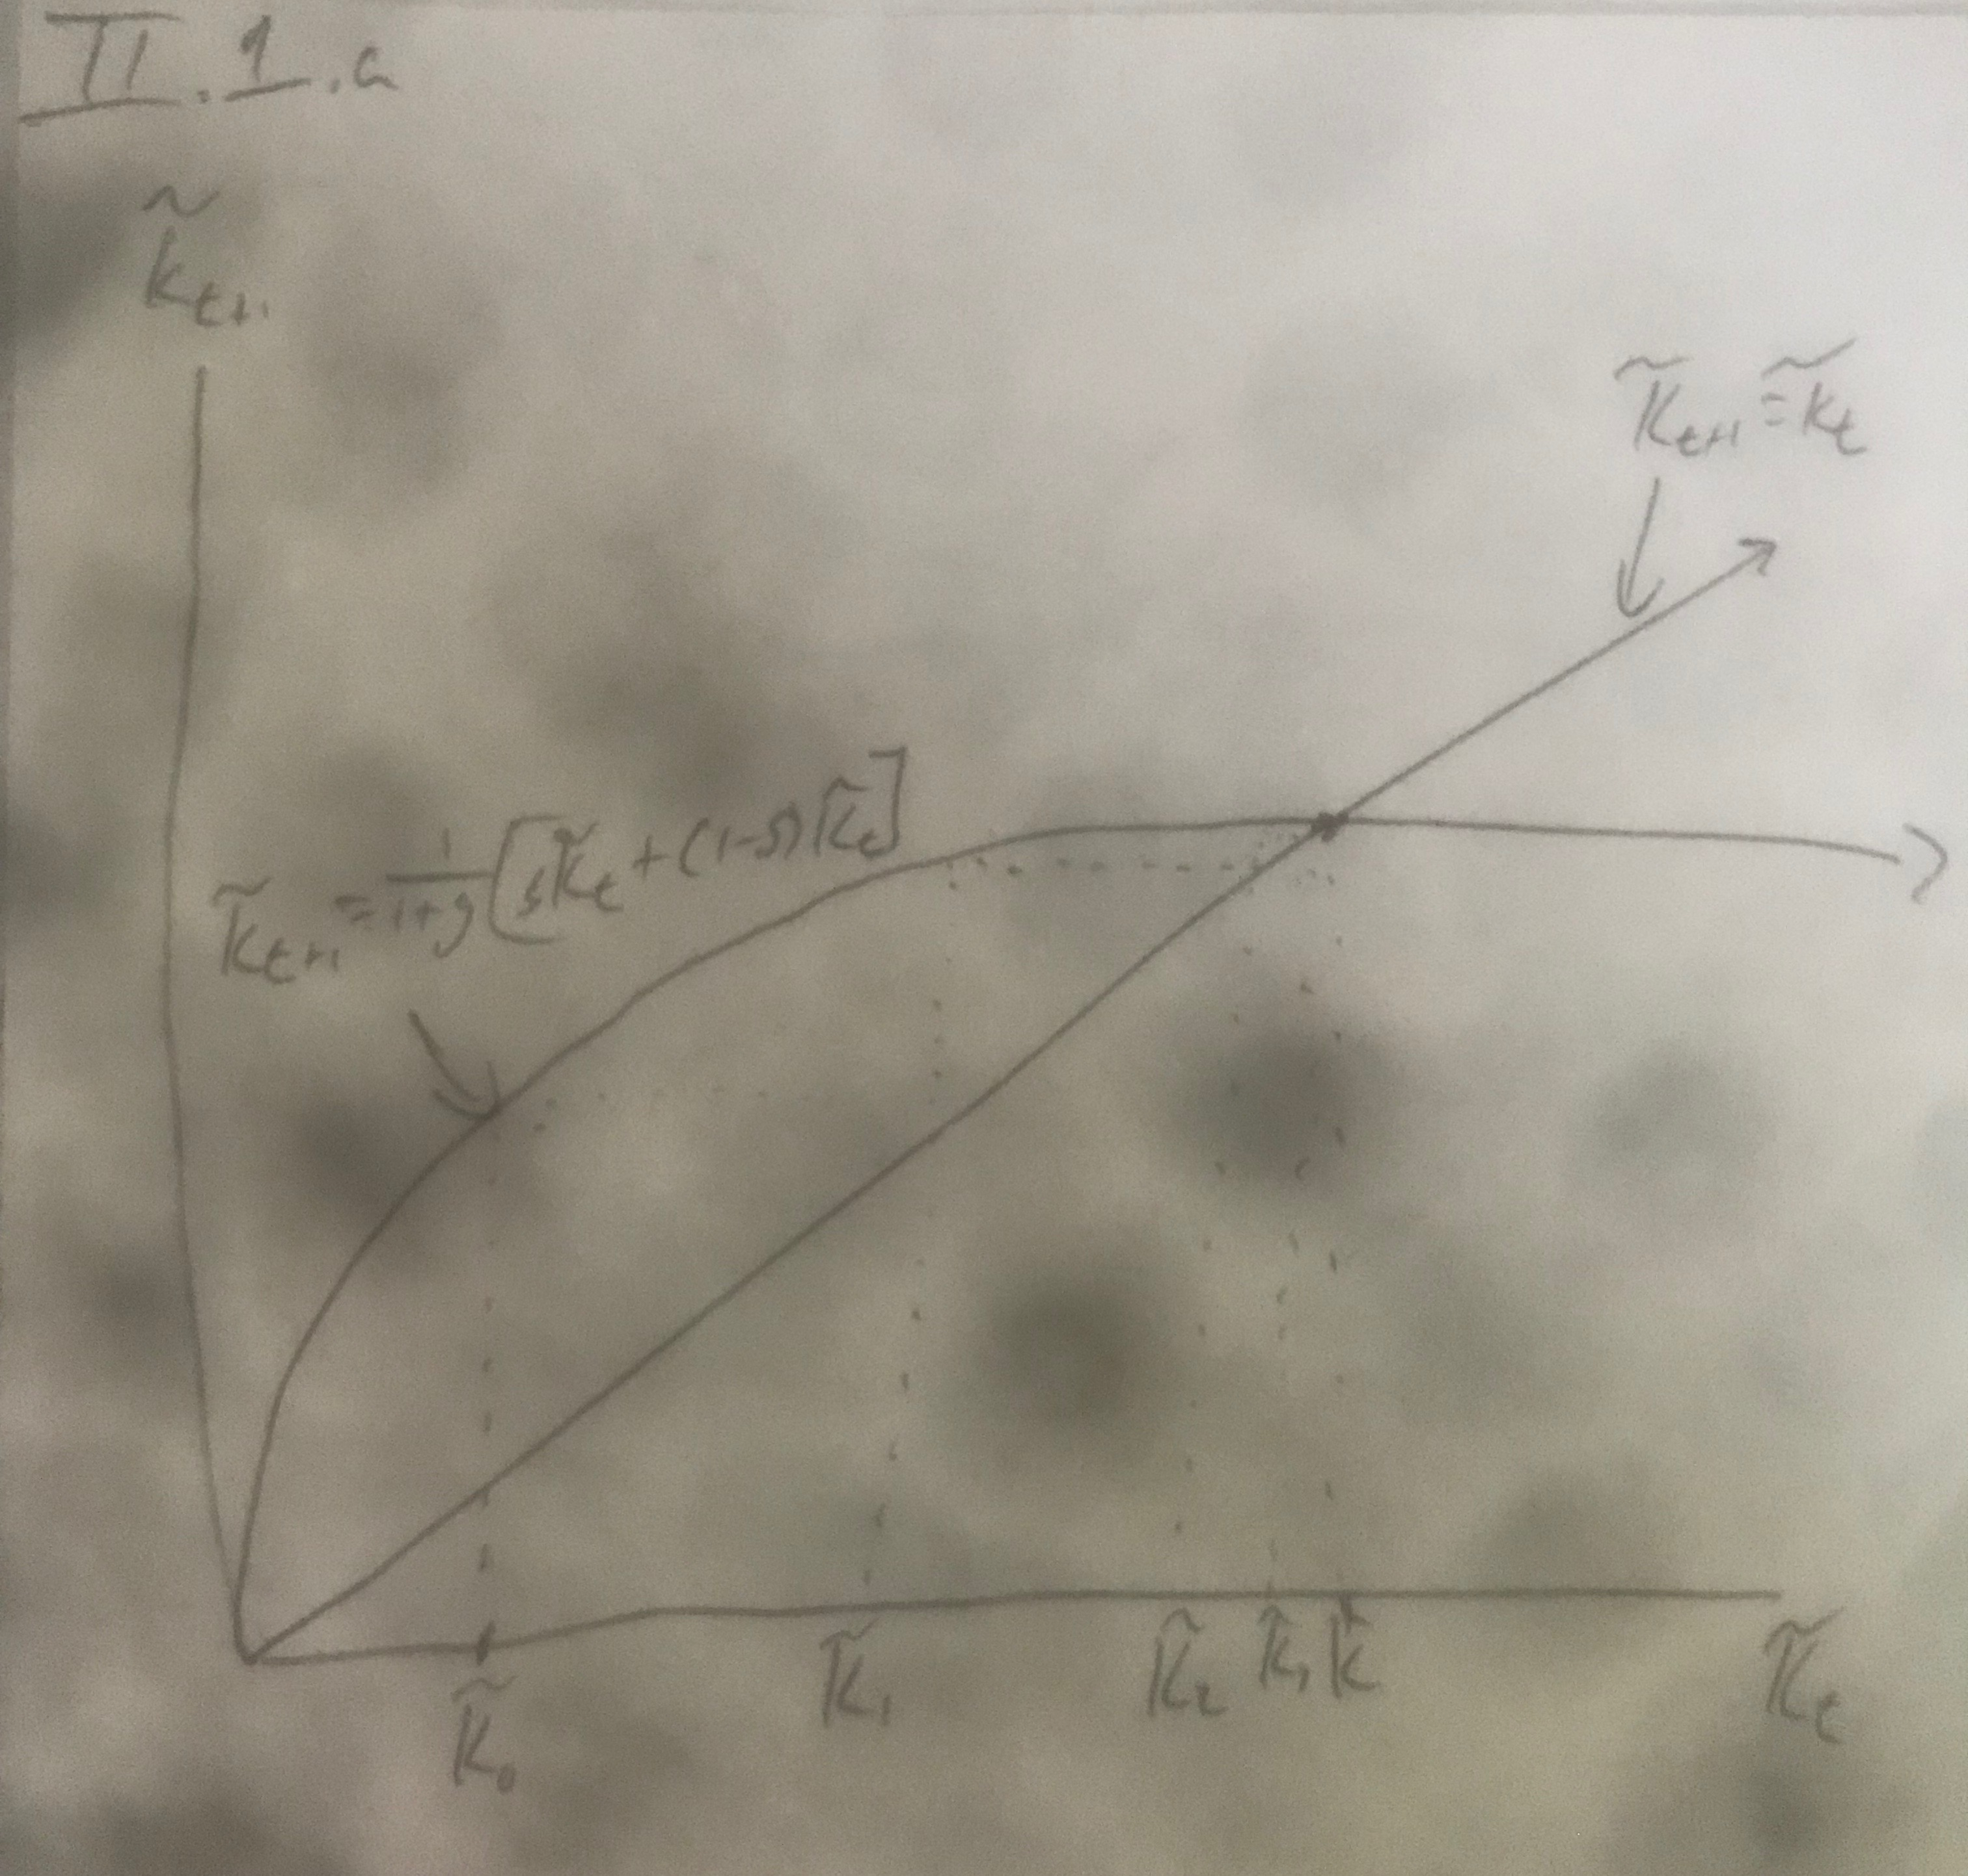
\includegraphics{graph1a.png}
  \end{figure}

\newpage
\clearpage
\noindent \textbf{Graph II.1.b}
\begin{figure}[h]
  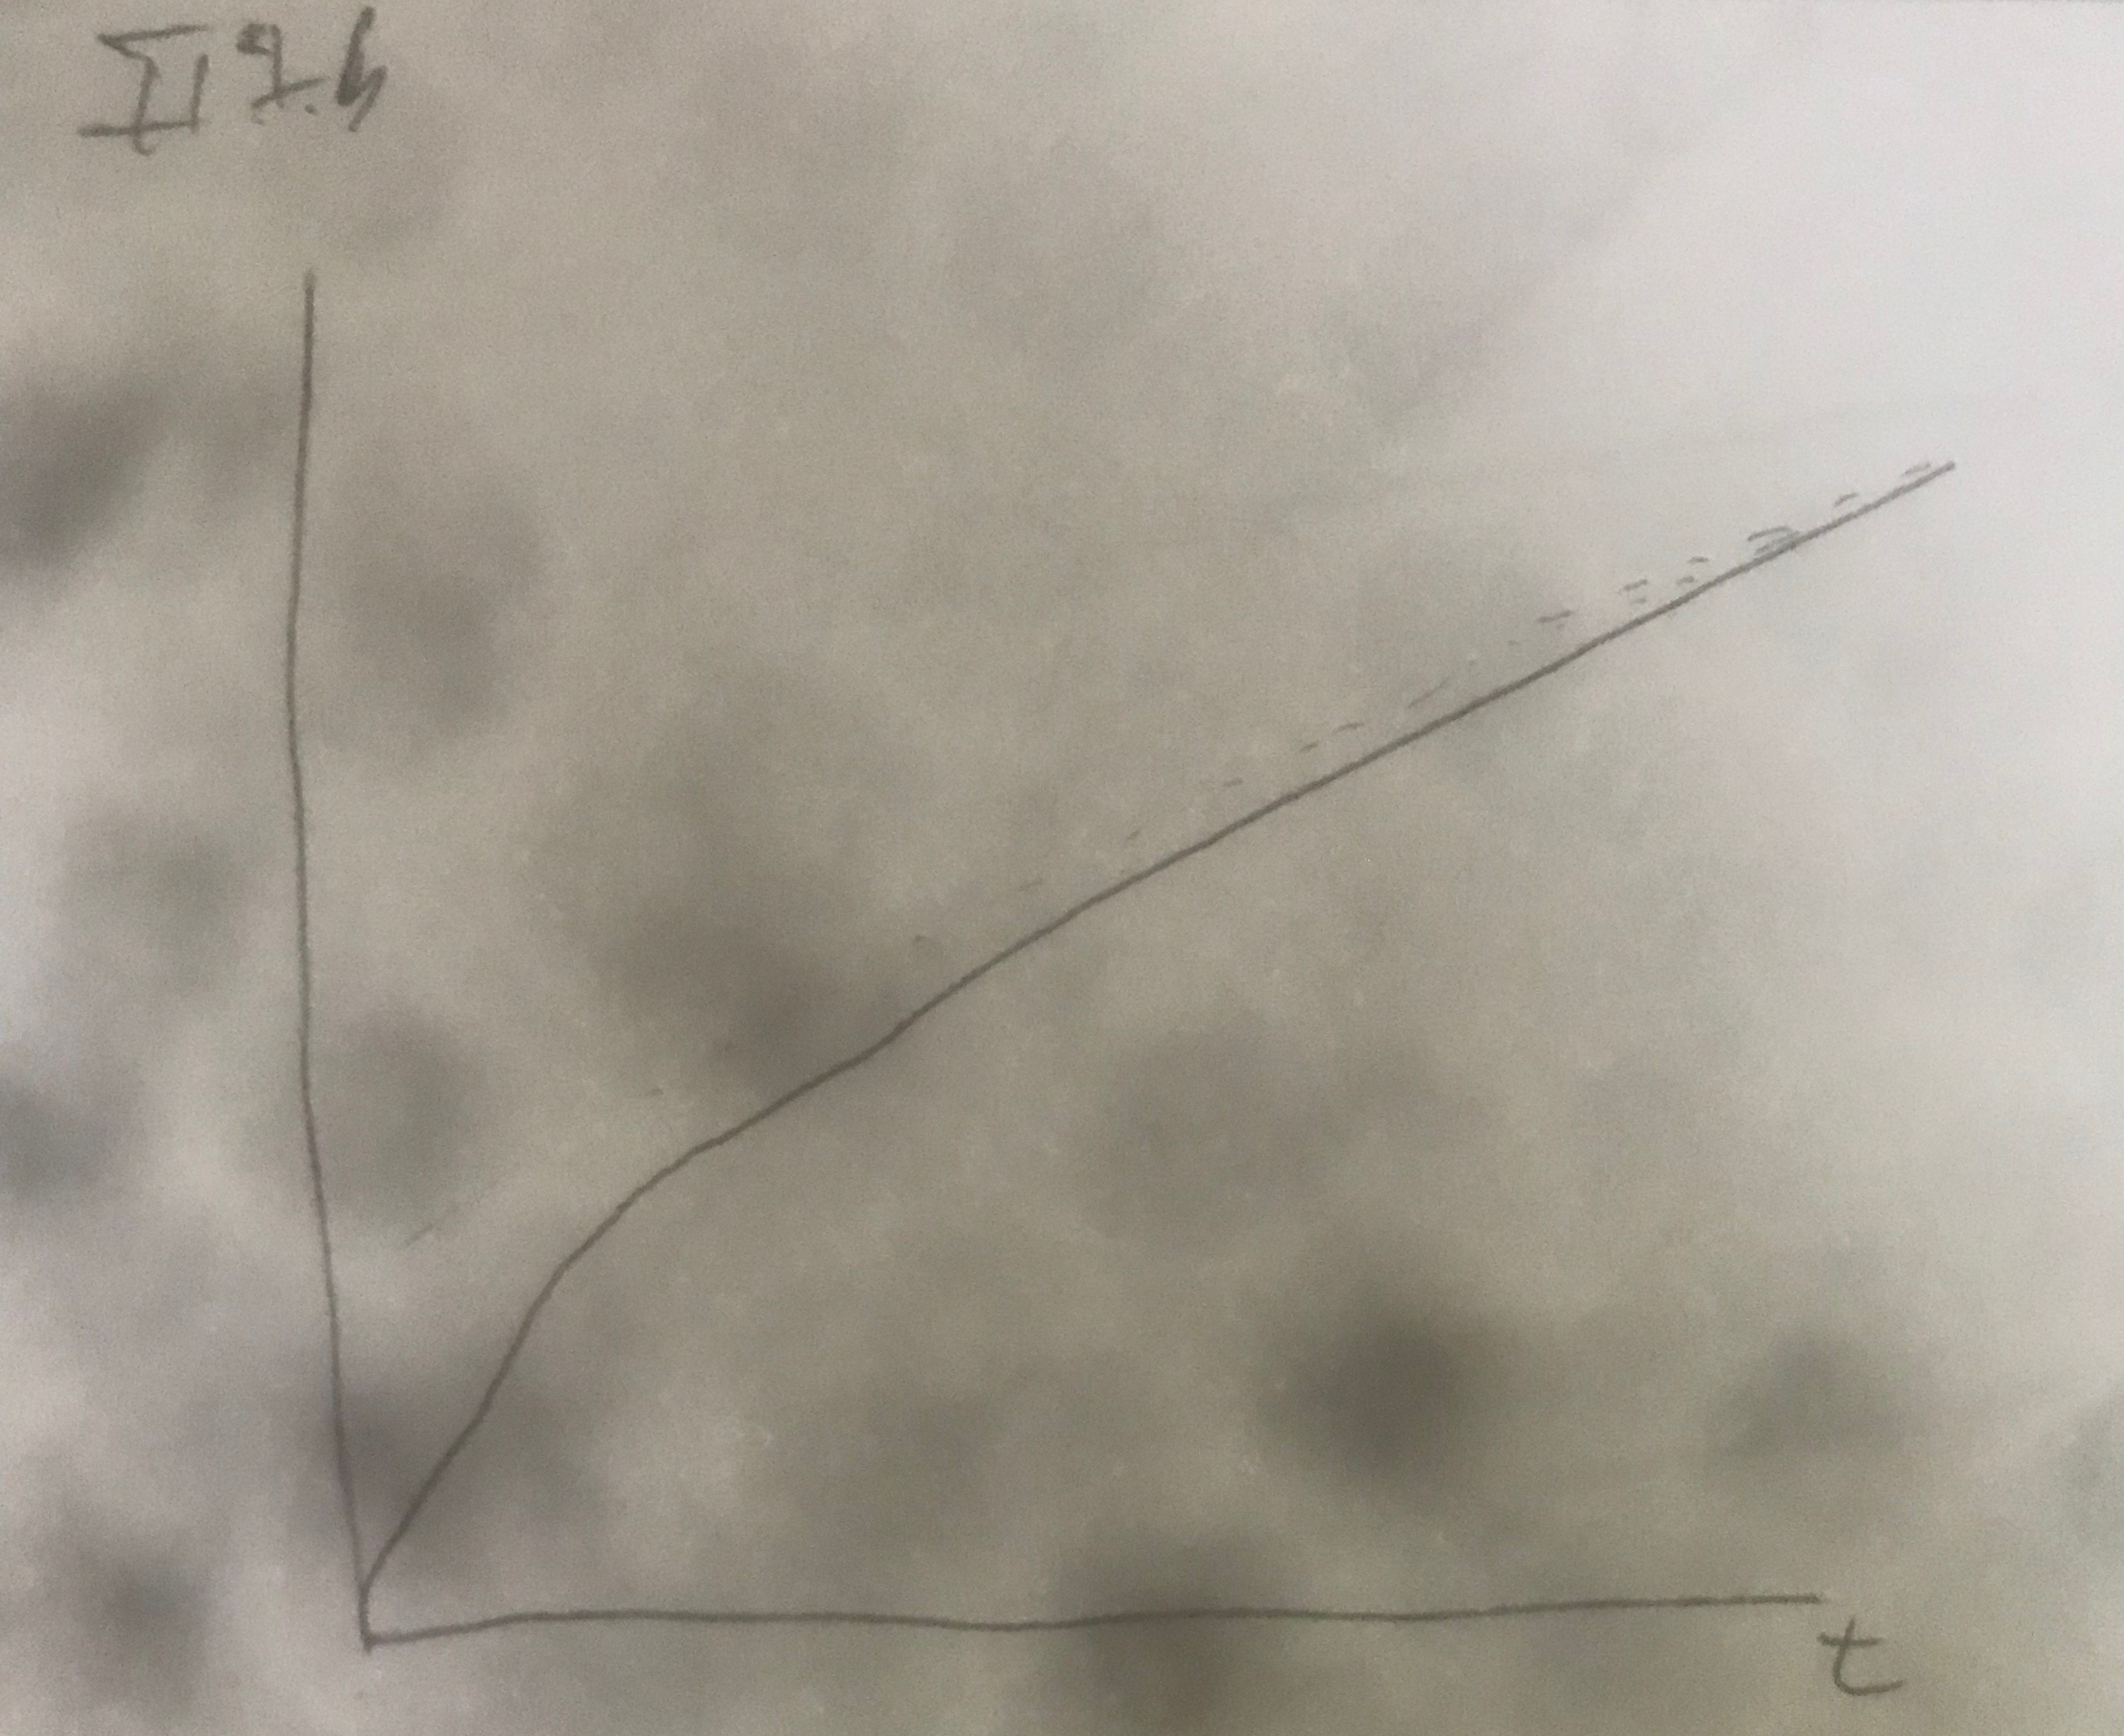
\includegraphics{graph1b.png}
  \end{figure}

\newpage
\clearpage
\noindent \textbf{Graph II.2}
\begin{figure}[h]
  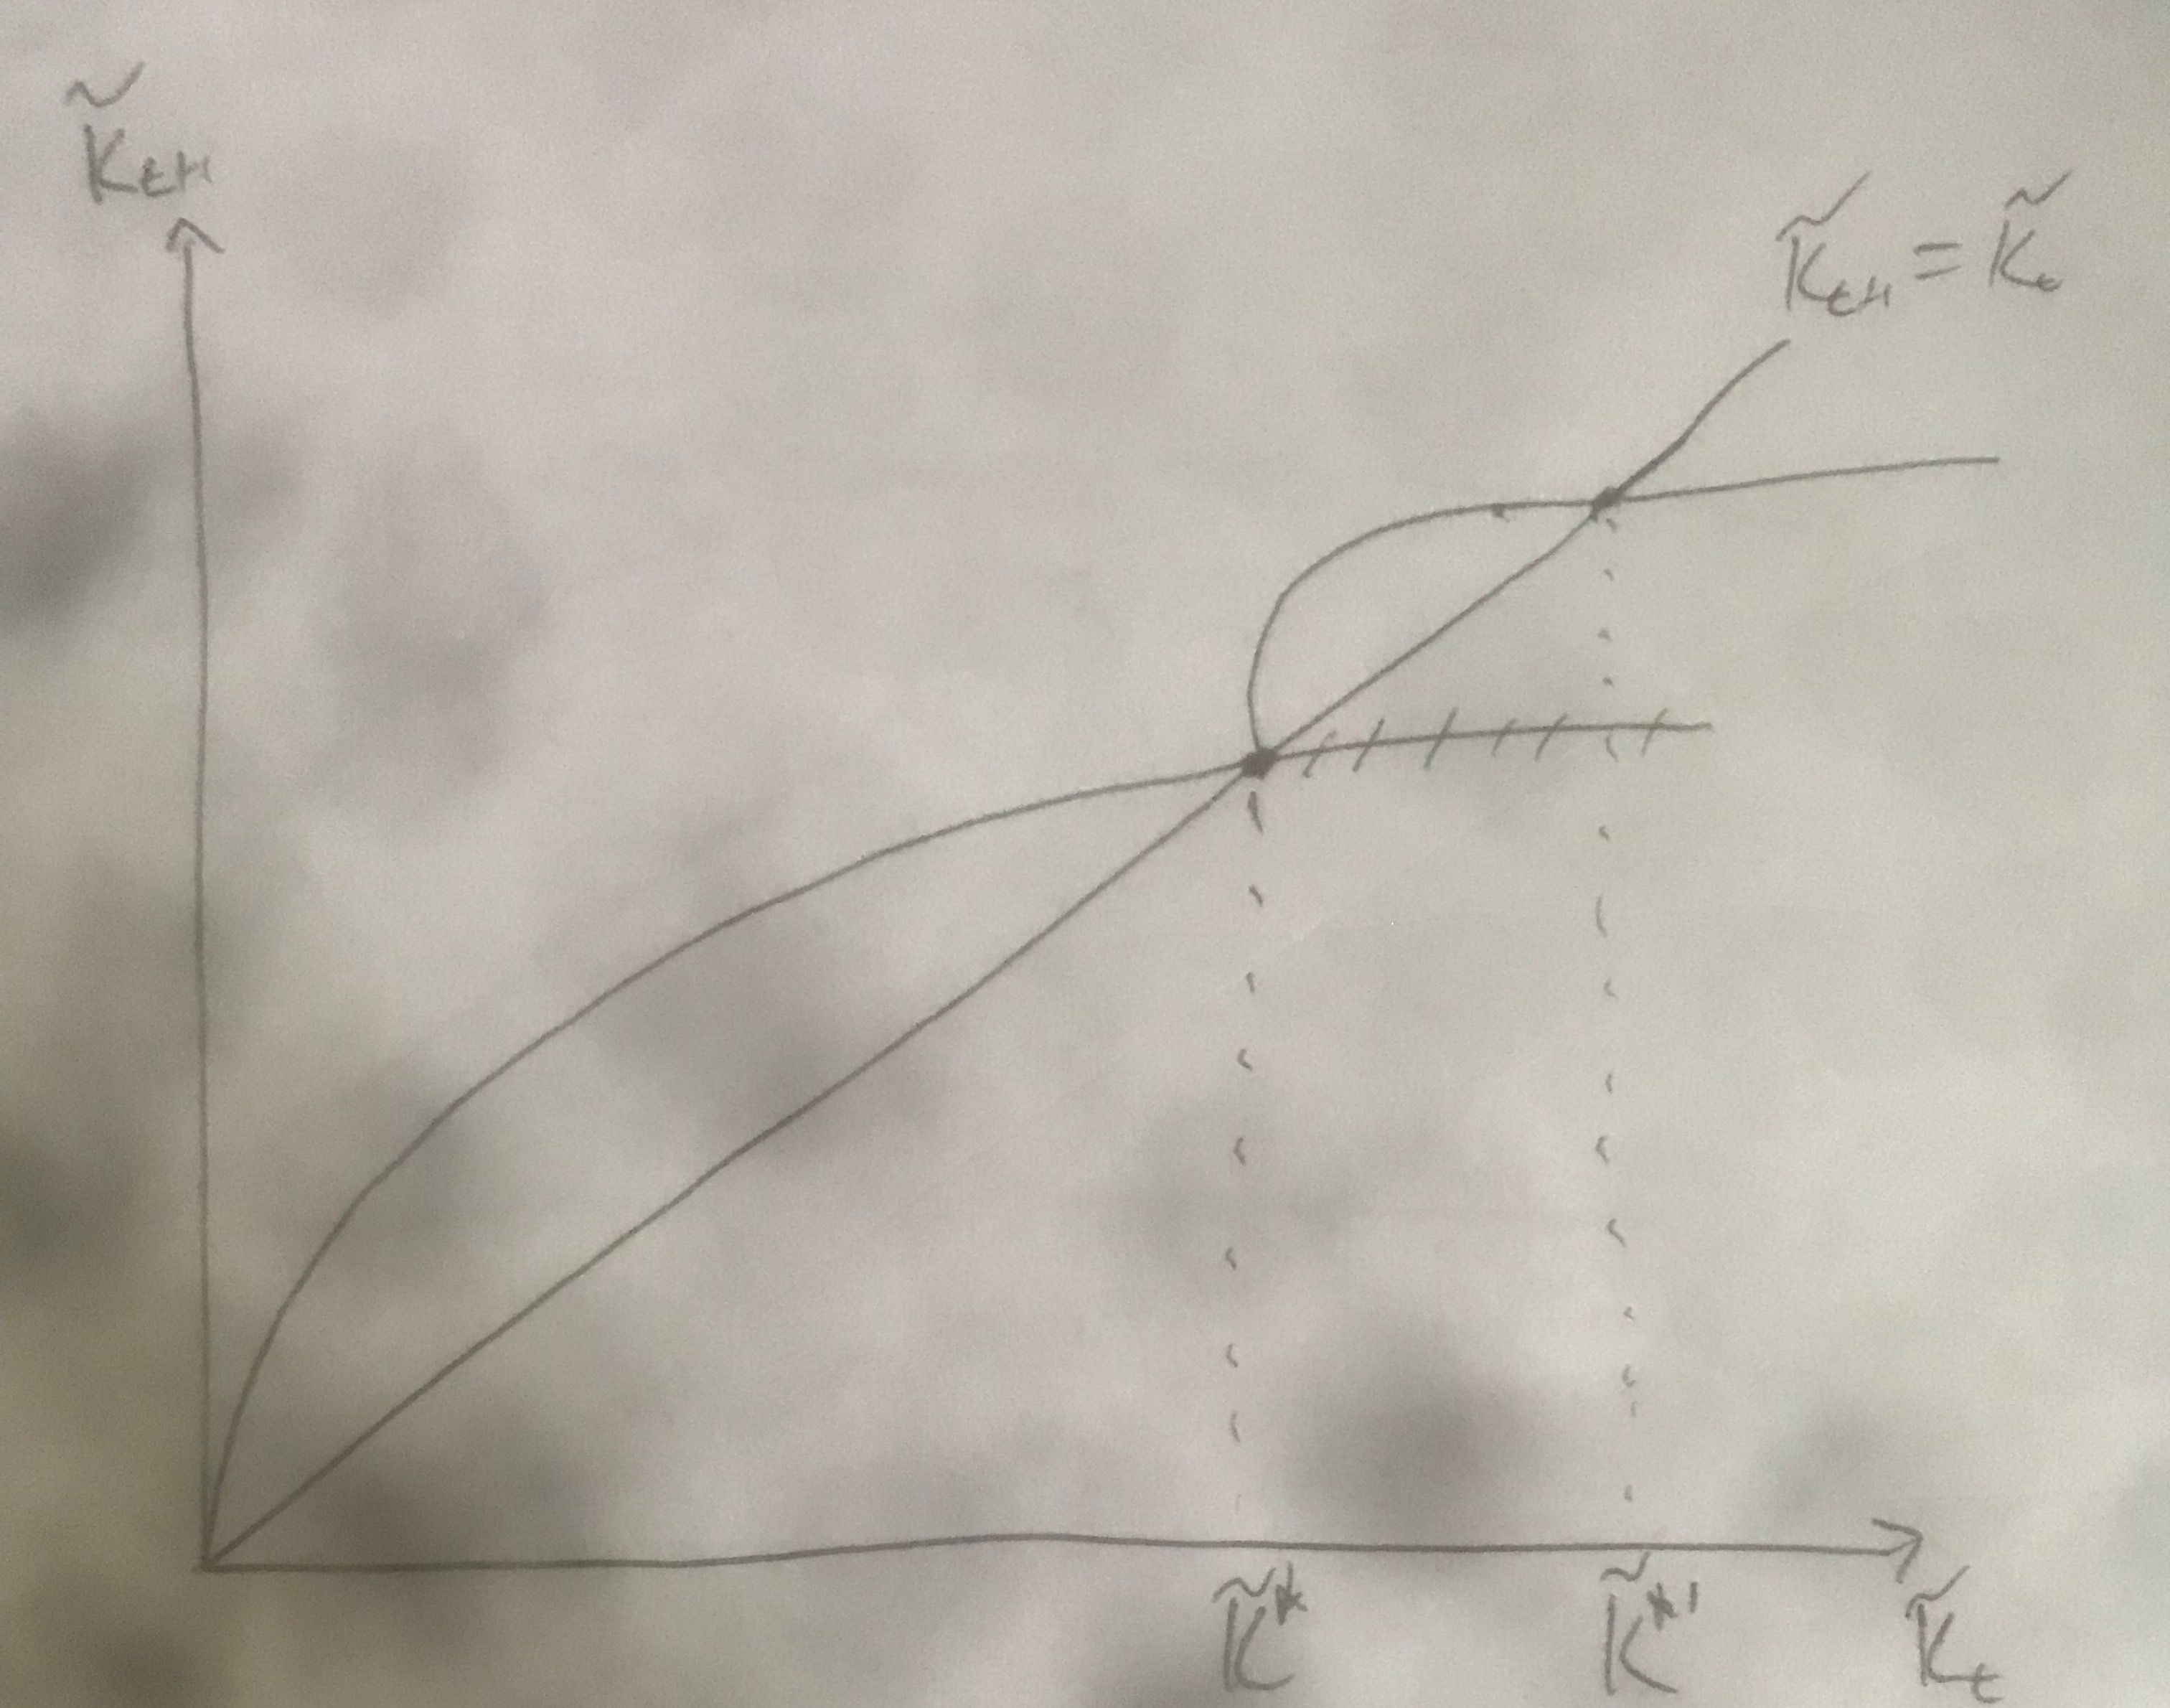
\includegraphics{graph2.png}
  \end{figure}

\newpage
\clearpage
\noindent \textbf{Graph II.3}
\begin{figure}[h]
  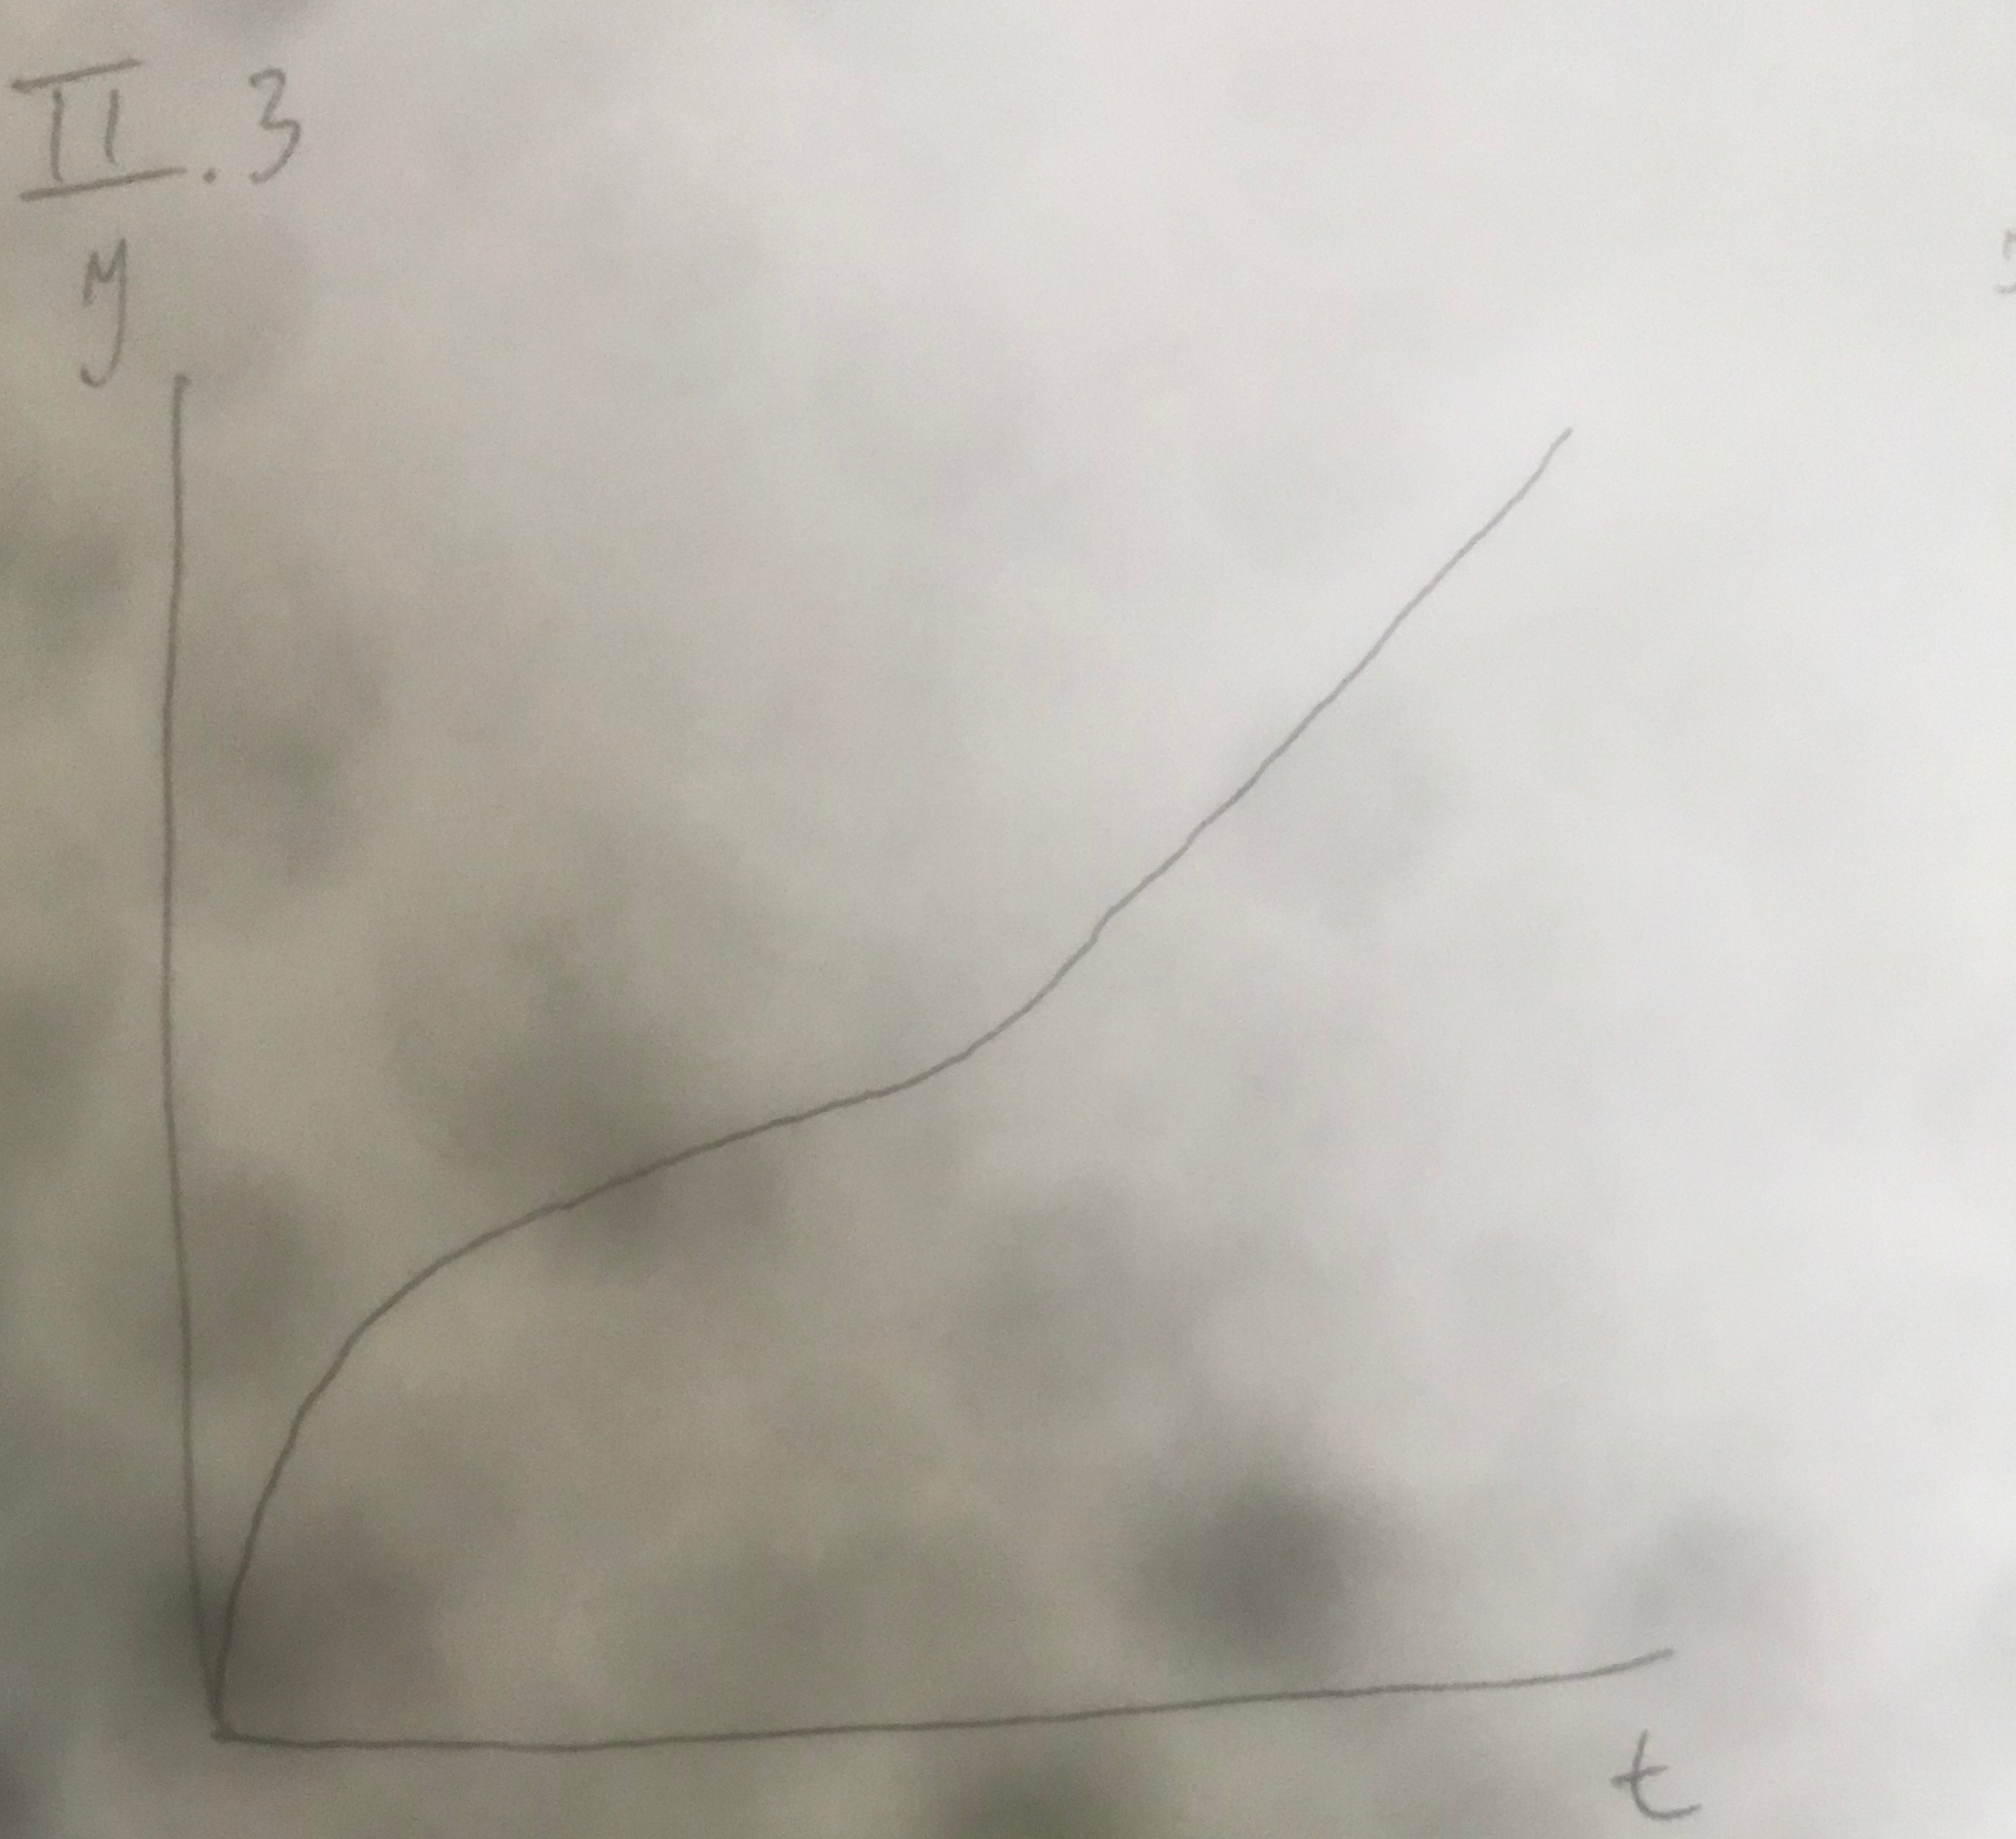
\includegraphics{graph3.png}
  \end{figure}
\end{document}